%Note one sentence in one text line for for better diffs.
\section{Measurement Results}
\label{sec:measurements}

Analysis of Apps.

We use the user agent field to classify the HTTP traffic. 

User agents have been previously used by \tbd{} to identify mobile devices.
Sites also use user agents to suggest users to access sites using their dedicated apps.
Applications use the user agent to identify themselves, along with the underlying operating system, software vendor, and software revision.
These identifiers are submitted with the help of an identification string sent with the HTTP requests made by the client.
We use this field to identify the applications. 
We filter out components of the underlying OS, device, and other version information. 
This filtering leaves us with the identifier of the applications along with other strings. We then use the edit distance to cluster these tokens and group the user agents according to the applications. 
Using this technique we were able to classify   




\tbd{In this section we ... }

\subsection{Descriptive Statistics}  

We now use several descriptive statistics to summarize our \moball dataset.
We use these descriptions to support our claim that \platname can be used as a portable, pervasive, and deployable platform for passive measurements of mobile network traffic. 

\subsubsection{Comparison of Devices} 
% Why this is important
One advantage of using \platname is that we can detail and compare the behavior of mobile devices regardless of the underlying operating system. 
We now use \fref{tab:summaryIOSAndroidTraffic} to directly compare Android and iOS, focusing on the key protocols used by the devices. 

% What we see HTTP and SSL, UDP, and other
Our first key observation is that HTTP is responsible for the majority TCP traffic volume in bytes, \tbdv{63.13\%} for Android and \tbdv{80.28\%} for iOS. 
This observation is inline with previous results that report HTTP to be the dominant protocol used by mobile devices~\cite{falaki:mobileusage, maier:mobtraffic}. 
We also observe that the majority of TCP flows are sent over SSL,  \tbdv{43.77\%} of total flows for Android and \tbdv{32.18\%} of total flows for iOS . 
We believe this occurs across platforms because the majority of flows come from e-mail, messaging and social networking, all of which use secure channels regardless of the OS. 
We discuss some of these popular application in \tbd{section}.

For the Android devices in the \moball dataset, \tbdv{96.45\%} of the UDP flows that account for \tbdv{70.92\%} of the UDP bytes are due to DNS request. 
The rest of the traffic is due to other applications such as Skype. 
Similarly, \tbdv{80.98\%} of UDP flows that account for \tbdv{66.29\%} of UDP bytes from iOS devices are due to DNS requests. 

We observe 0.1\% of the traffic volume was classified as \emph{other} for Android device which is larger than the 0.01\% observed for iOS. 
This is because the Android users in our dataset tend troubleshoot network connectivity issues using applications that perform pings and traceroutes. 

% Other insights not present in the table
On balance the number of bytes transferred per unit time in Android, and the number of flows, is larger than the same for iOS. 
We found that iOS devices generated about \tbdv{number} of traffic per hour while Android devices generated about\tbd{number} MB/hr, and increase of \tbdv{number\%}.
Further, Android devices contributed more flows (\tbdv{number} per hour vs. \tbdv{number} per hour), an  increase of \tbdv{40\%}. 
It is difficult to account for the impact of   user behavior on device-generated traffic; that aside, one explanation is that Android devices generate more bytes and flows due to the relatively permissive API for running code in the background on Android. 
In contrast, iOS quickly kills processes that are in the background, preventing them from  generating network traffic after only a few seconds of losing the foreground. 
We discuss this \tbd{section}

%Why this is important
\tbd{In summary, }

\begin{table}
\begin{center}
\begin{small}
\begin{tabular}{|l|l|r|r|r|r|}
\hline
\multirow{2}{*}{\bf Protocol} & \multirow{2}{*}{\bf Service} & \multicolumn{2}{|c|}{\bf Android} & \multicolumn{2}{|c|}{\bf iOS} \tabularnewline
\cline{3-6}
           &           &  \textbf{Flows}  &  \textbf{Bytes}  &  \textbf{Flows}  &  \textbf{Bytes}  \tabularnewline
\hline
 TCP       &  HTTP     &  13.55  &  63.13  &  14.64  &  80.28  \tabularnewline
\hline
TCP       &  SSL      &  43.77  &  31.36  &  32.18  &  18.98  \tabularnewline
\hline
 UDP       &  -        &  37.23  &   1.09  &  47.32  &   0.55  \tabularnewline
\hline
 TCP       &  other    &   2.24  &   4.30  &   1.55  &   0.15  \tabularnewline
\hline
 Other     &  -        &   3.19  &   0.10  &   4.03  &   0.01  \tabularnewline
\hline
\multicolumn{2}{|c|}{\emph{total}} & 100.00 & 100.00 & 100.00 & 100.00 \tabularnewline
\hline
\end{tabular}
\end{small}
\end{center}
\caption{Percentage of flows and bytes from iOS and Android devices.
\tbd{Verify total 100 for final results} \emph{SSL is responsible for the
majority of TCP flows from iOS and Android devices.}}
\label{tab:summaryIOSAndroidTraffic}
\end{table}

\subsubsection{Comparison of Access Technology}
% Why this is important
\platname allows us to passively monitor traffic regardless of the access technology used by the mobile device. 
We use this feature of \platname to provide a direct comparison of how the different access technologies are used by our users. 



\begin{figure}
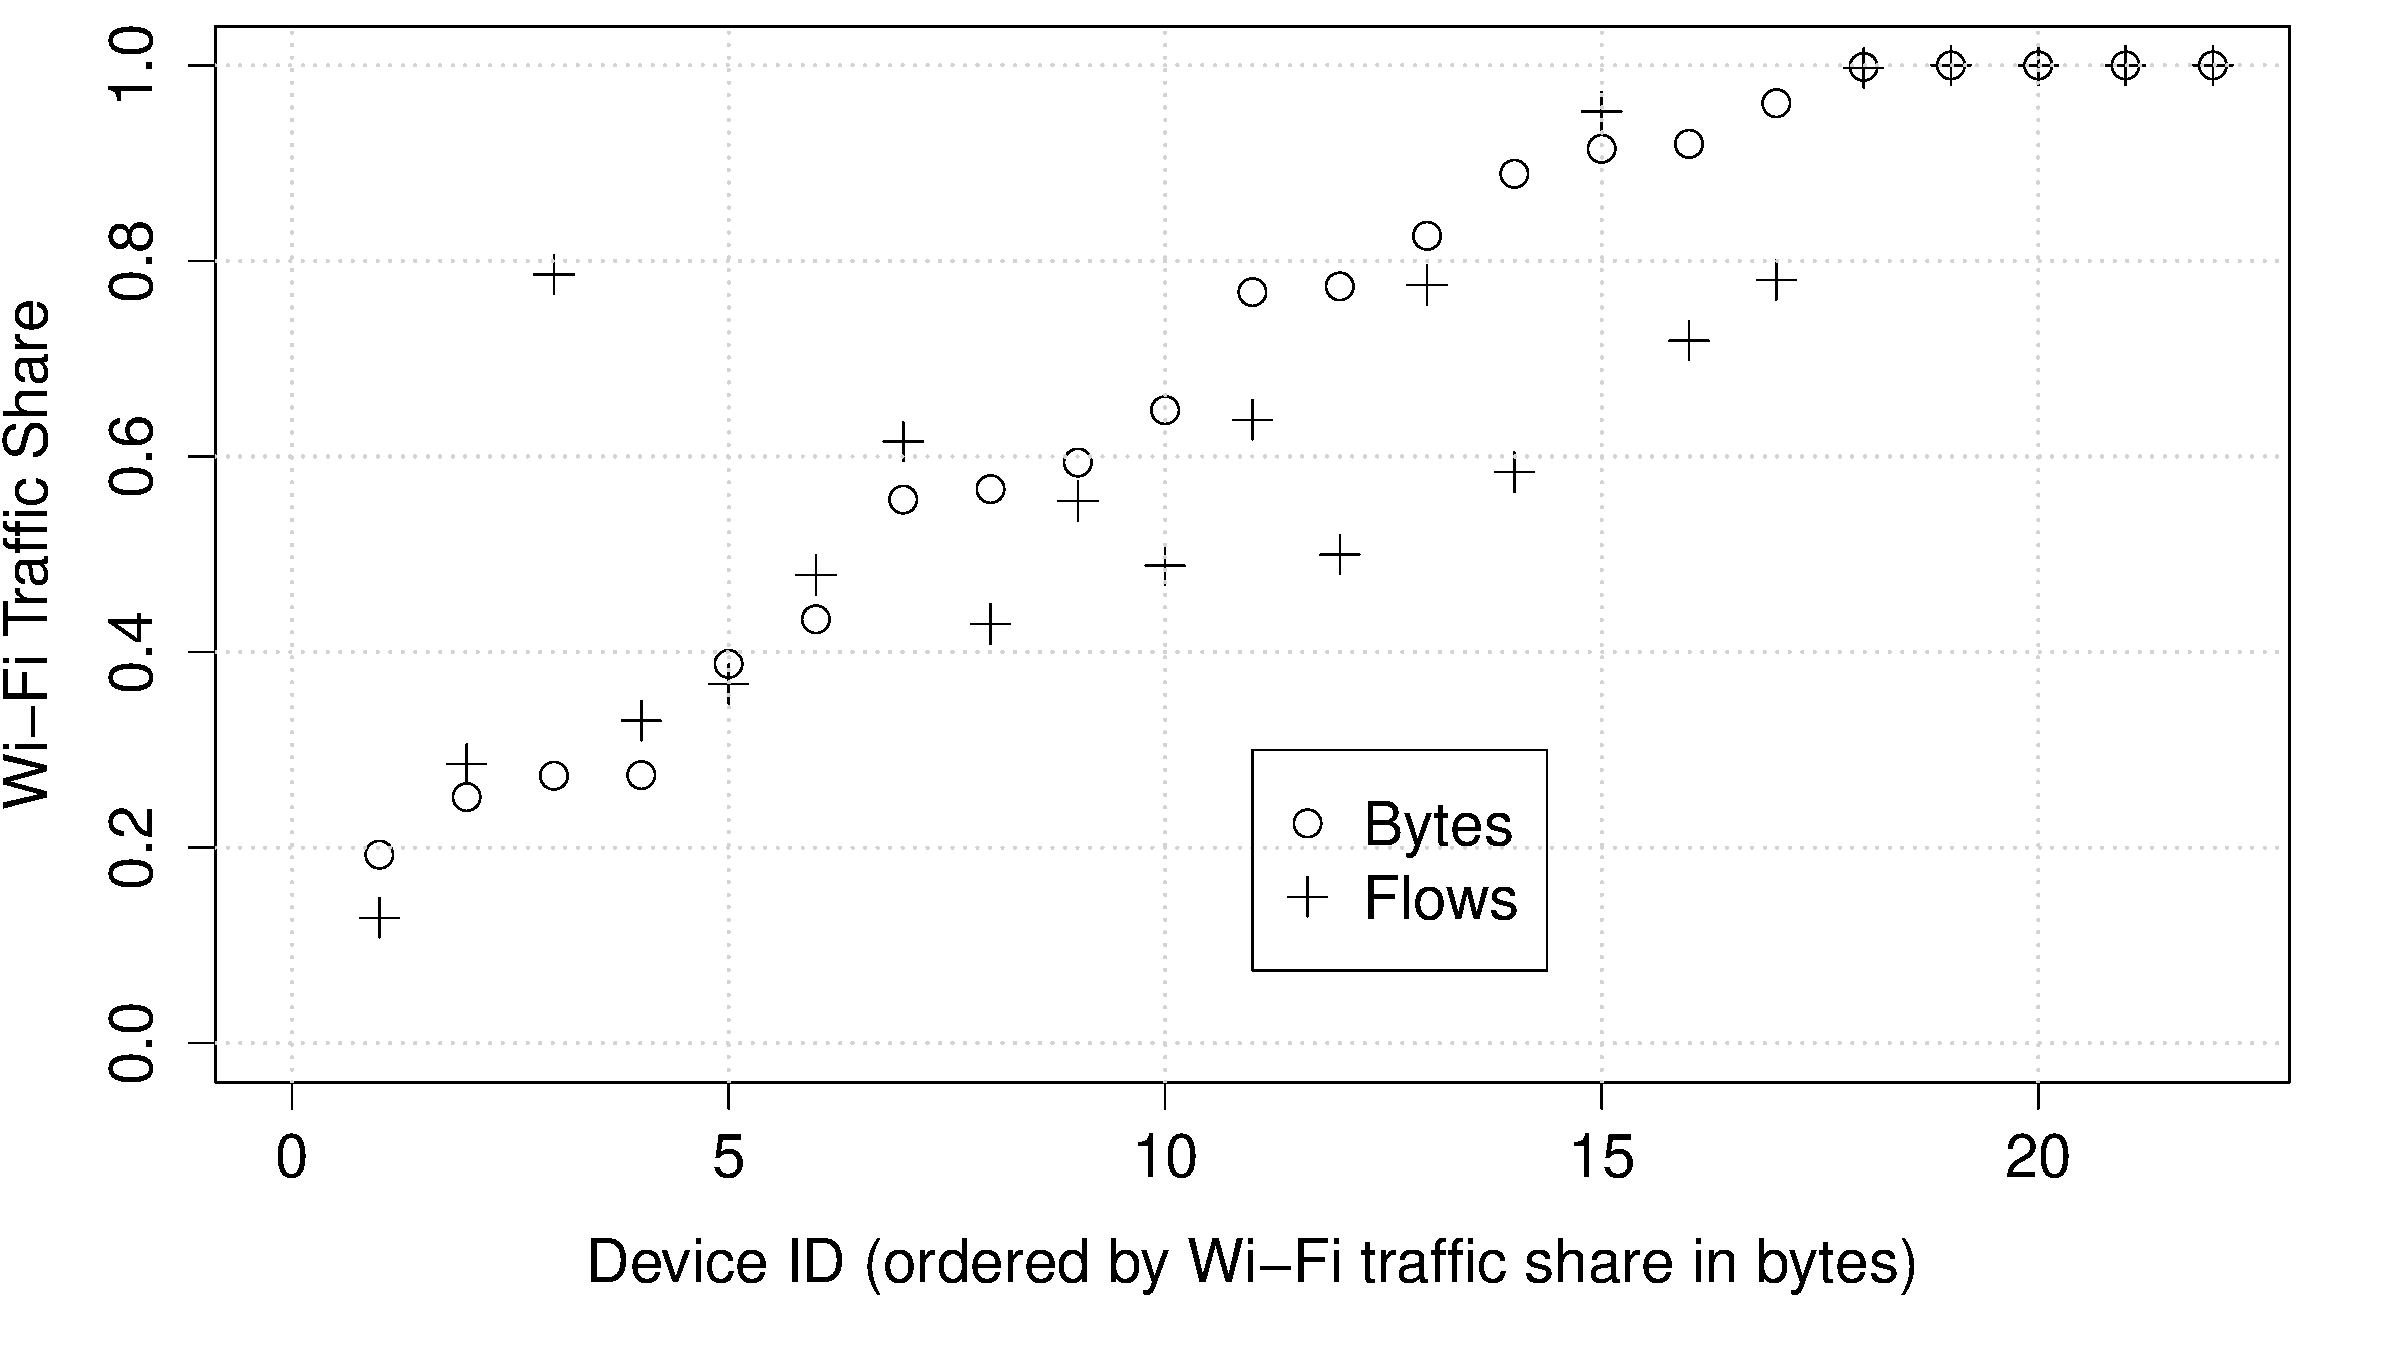
\includegraphics[width=\columnwidth]{plots/deviceTechShare.pdf}
\caption{Traffic share of \wifi as a fraction of total traffic from a device. }
\label{fig:devicetechshare}
\end{figure}

% What we observe
In \fref{fig:devicetechshare} we present the share of \wifi as a fraction of the total traffic generated by the user.
The devices are sorted according to the share of \wifi traffic as a fraction of the total traffic from the device.  
The devices with device IDs from \tbdv{18} to \tbdv{23} are devices that do not have a cellular data plan associated with them device: \tbdv{3} iPads, \tbdv{1} iPodTouch, and \tbdv{1} Android tablet.
The diversity in Wi-Fi traffic share in terms of flows and bytes indicates the diversity of mobile device usage. 
For example, device ID \tbdv{3} is used by a user who prefers to use cellular network to listen to music, watch videos, and troubleshoot the cellular network connectivity issues using tools such as speedtest; the primary use of the device is used to read emails and access social networks when on Wi-Fi. 
Media content such as music and videos have a higher share of traffic volume per flow, therefore the share of cellular traffic in higher for device ID \tbdv{3}. 
Similarly, device ID \tbdv{1} is used by a user who prefers to use cellular networks. 

\begin{table}
\begin{center}
\begin{small}
\begin{tabular}{|l|l|r|r|r|r|}
\hline
\multirow{2}{*}{\bf Protocol} & \multirow{2}{*}{\bf Service} & \multicolumn{2}{|c|}{\bf Wi-Fi} & \multicolumn{2}{|c|}{\bf Cellular} \tabularnewline
\cline{3-6}
           &           &  \textbf{Flows}  &  \textbf{Bytes}  &  \textbf{Flows}  &  \textbf{Bytes}  \tabularnewline
\hline
 TCP       &  HTTP     &  16.14  &  81.59  &  10.99 &  57.08\tabularnewline
\hline
 TCP       &  SSL      &  32.56  &  16.97  &  43.99 &  39.59 \tabularnewline
\hline
UDP       &  -        &  46.29  &   0.52  &  38.56  &  1.25  \tabularnewline
\hline
TCP       &  other    &   1.43 &   0.89  &   2.46  &   1.97  \tabularnewline
\hline
Other     &  -        &   3.55 &  0.02  &   3.96 &   0.09  \tabularnewline
\hline
\multicolumn{2}{|c|}{\emph{total}} & 100.00 & 100.00 & 100.00 & 100.00 \tabularnewline
\hline
\end{tabular}
\end{small}
\end{center}
\caption{Percentage of flows and bytes using Wi-Fi and Cellular as access technology. \tbd{Verify total 100
    for final results} \emph{The share of SSL traffic over Cellular
    networks is larger than its share over Wi-Fi in terms of bytes and flows}}
\label{tab:summaryWifiCellularTraffic}
\end{table}

In \fref{tab:summaryWifiCellularTraffic} we further classify the protocols and services that are responsible for \wifi and cellular data traffic with the help of the techniques used to generate \fref{tab:summaryIOSAndroidTraffic}. 
The first key observation is that the portion of HTTP bytes sent over \wifi and cellular are significantly different. 
Upon further inspection, we found that Wi-Fi is the preferred medium to transfer media content, which generates relatively large flows. 
For example, apps such as Google Plus image backup on Android allow users to upload their
images only over Wi-Fi. 
In line with the difference in HTTP traffic ratios, we note that SSL flows are dominant type in cellular connections. 
We also observe a smaller number of UDP flows for cellular networks. 
\tbd{Why do we observe less??}.

\begin{figure}
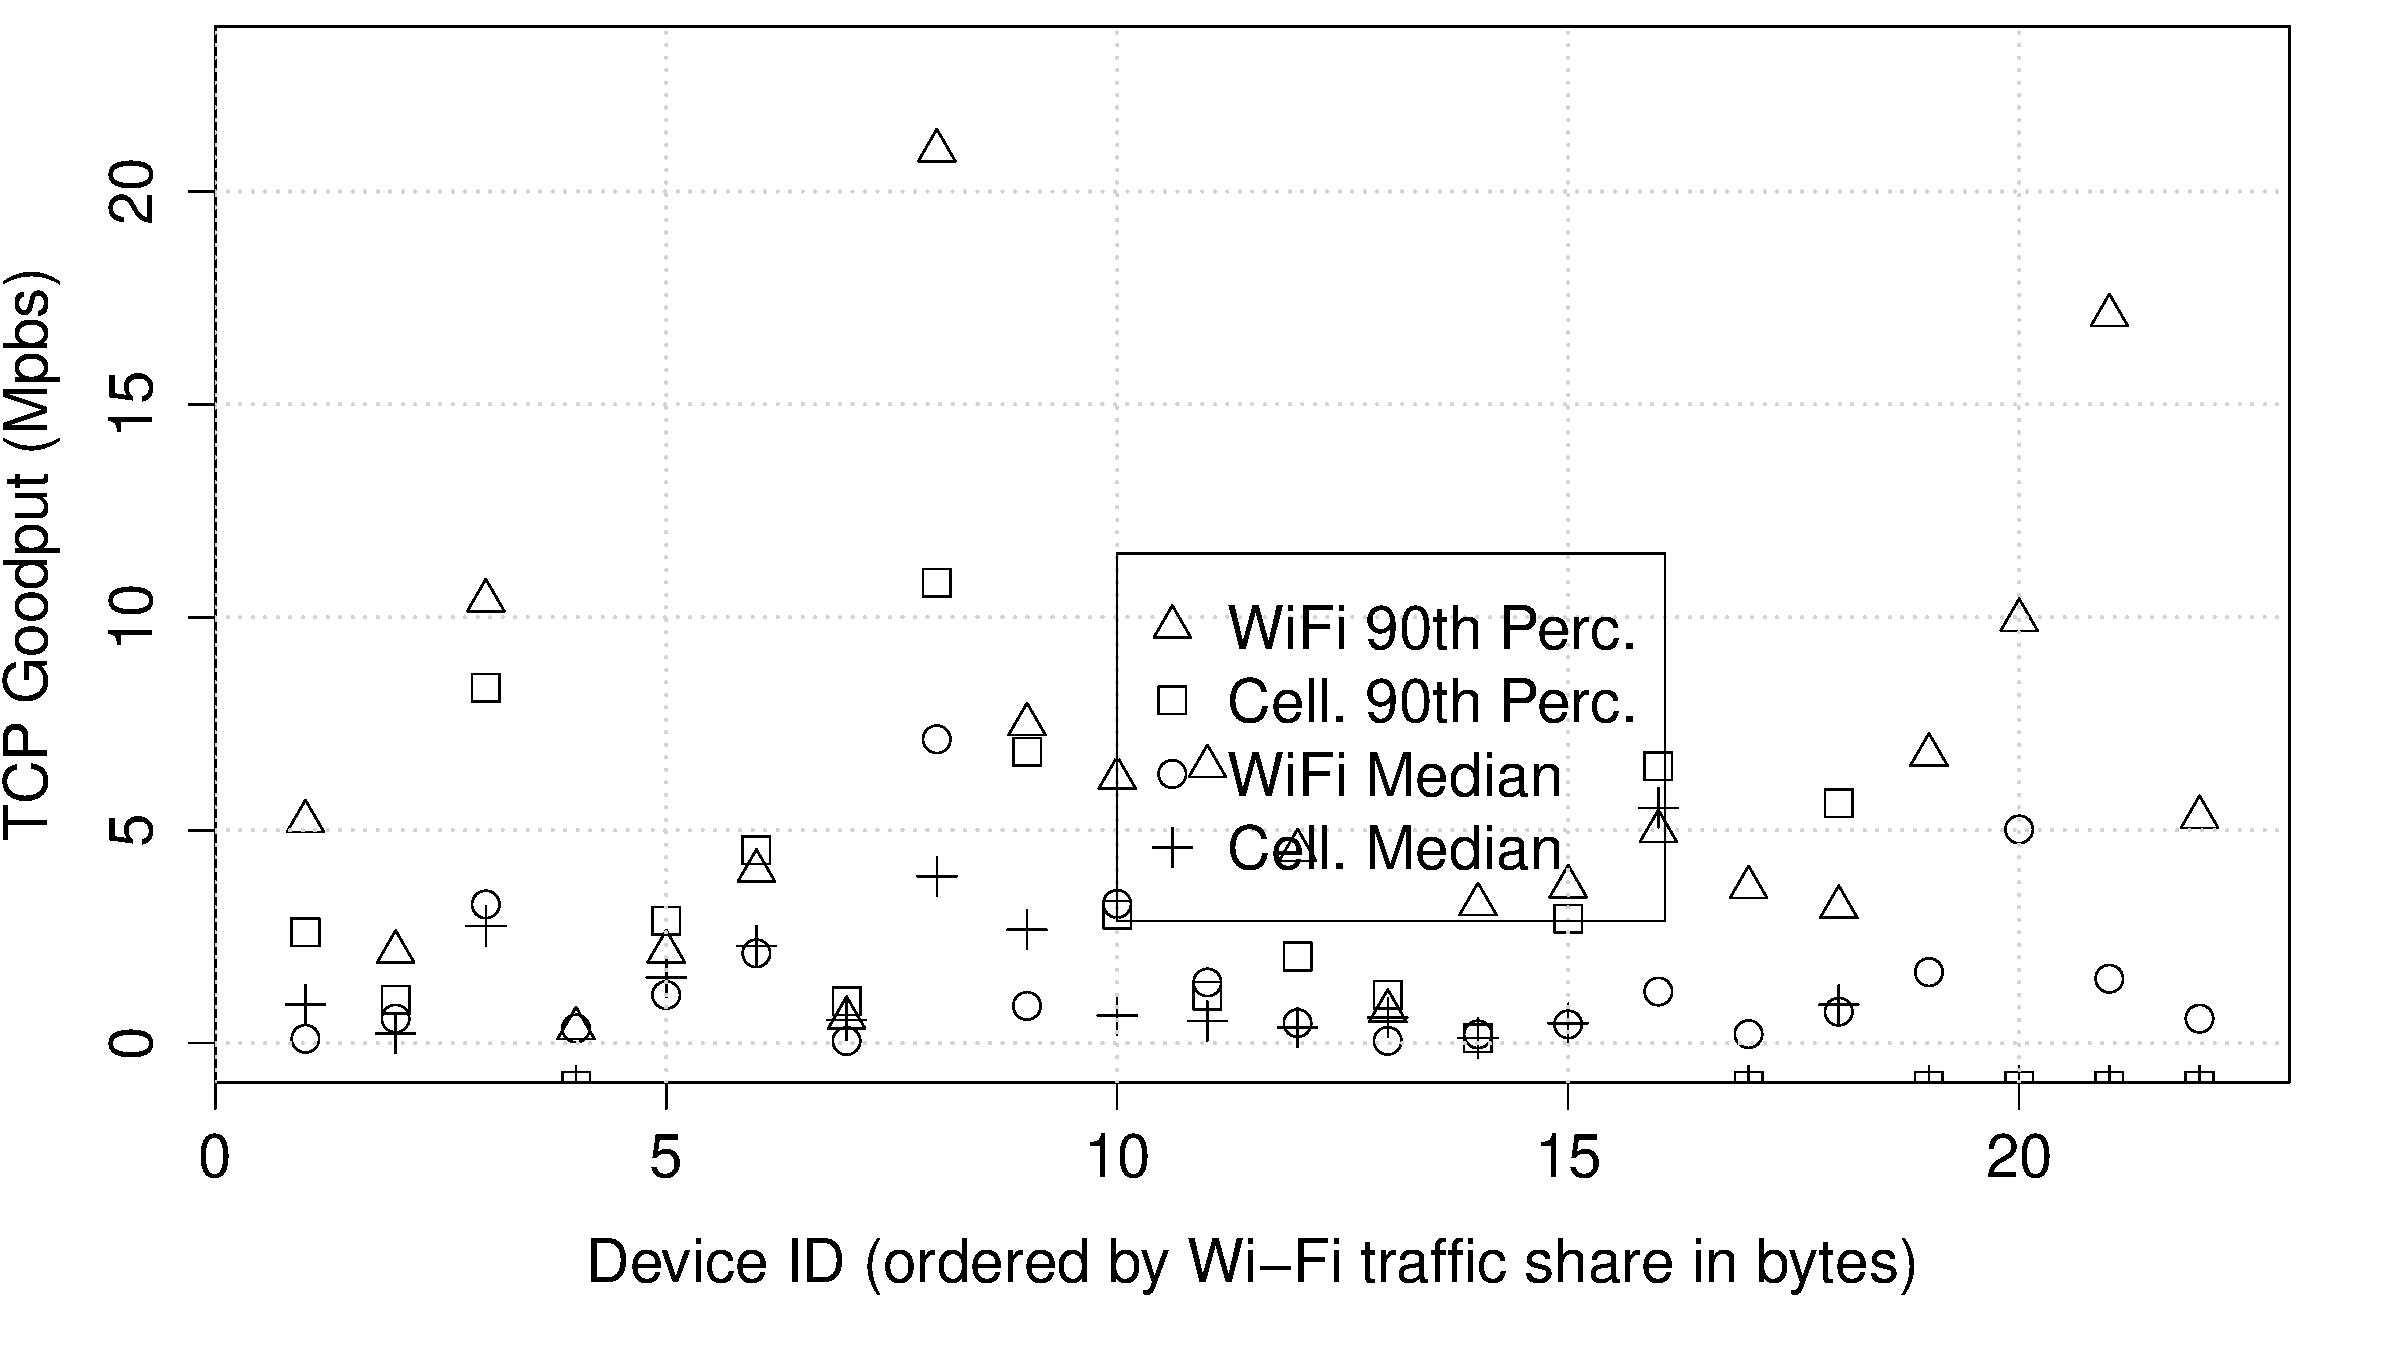
\includegraphics[width=\columnwidth]{plots/deviceTechDataRate.pdf}
\caption{Goodput of TCP flows over \wifi and cellular networks.}
\label{fig:devicetechrate}
\end{figure}

In \fref{fig:devicetechrate}, we present the 90th percentile and median TCP goodput of flows that exchanged more than 512~kB of data.
\tbd{cite ~\cite{httparchive} if needed for 256 kB}.
We use the goodput because it a good estimate of how the applications perceive the quality of the network.  
The devices are sorted according to the same technique used to sort the devices in \ref{fig:devicetechshare}.
For device 16 we observe higher goodput for cellular compared to \wifi while for device 6 we observe similar values for the 
TCP goodput; this highlights opportunities for proposals such as 3G onloading~\cite{vr:3gol}.
Across all users we observe that ratio of median goodput over \wifi to the median goodput over cellular varies from \tbdv{ } to \tbdv{ } with a median of \tbdv{}.

% discussion
\tbd{In summary, }


\subsection{Case Studies}


\subsection{Controlled Experiments}

\subsection{Discussion}

%%% Local Variables: 
%%% mode: latex
%%% TeX-master: "main"
%%% End: 




